% This file should be built with xelatex, not the standard latexmk.

\documentclass[conference]{IEEEtran}
\IEEEoverridecommandlockouts
% The preceding line is only needed to identify funding in the first footnote. If that is unneeded, please comment it out.
\usepackage{cite}
\usepackage{amsmath,amssymb,amsfonts}
\usepackage{algorithmic}
\usepackage{graphicx}
\usepackage{textcomp}
\usepackage{xcolor}
\usepackage{multirow}
\usepackage{tabularx}
\usepackage{listings}
\usepackage{color}

% This didn't work for Russian...
% \usepackage[utf8]{inputenc} % Use UTF-8 encoding
% \usepackage[T2A]{fontenc}    % Enable Cyrillic font encoding
% \usepackage[russian]{babel}  % Load babel for Russian language support


\definecolor{dkgreen}{rgb}{0,0.6,0}
\definecolor{gray}{rgb}{0.5,0.5,0.5}
\definecolor{mauve}{rgb}{0.58,0,0.82}

\lstset{
  frame=tb,
  language=Python,
  aboveskip=3mm,
  belowskip=3mm,
  showstringspaces=false,
  columns=flexible,
  basicstyle=\ttfamily,
  columns=fullflexible,
  keepspaces=true,
  numbers=none,
  numberstyle=\tiny\color{gray},
  keywordstyle=\color{blue},
  commentstyle=\color{dkgreen},
  stringstyle=\color{mauve},
  breaklines=true,
  breakatwhitespace=true,
  tabsize=3,
  literate={
    {helloworldurdu} {{\urdufont سلام دنیا}}1
    {goodbyeurdu} {{\urdufont خدا ہافظ}}1
  }
}

% Enable multilingual typesetting
\usepackage{polyglossia}      % Supports multiple languages and their configurations
\setdefaultlanguage{english}  % Set main language to English
\setotherlanguage{urdu}       % Add Urdu as a secondary language

% Font setup for each language
\newfontfamily\urdufont[Script=Arabic,Scale=1.2]{Jameel Noori Nastaleeq} % Urdu font

\def\BibTeX{{\rm B\kern-.05em{\sc i\kern-.025em b}\kern-.08em
    T\kern-.1667em\lower.7ex\hbox{E}\kern-.125emX}}
\begin{document}

\title{UniversalPython - A Multilingual Python Programming Language*\\
{\footnotesize \textsuperscript{*}
Note: This draft was submitted in partial fulfillment of the requirements for the course "Research Methodology"
at FAST-NUCES

}
}

\author{\IEEEauthorblockN{Saad Ahmed Bazaz}
\IEEEauthorblockA{\textit{Software Engineering and Product Design} \\
\textit{Grayhat}\\
Islamabad, Pakistan \\
bazaz@grayhat.studio}
}

\maketitle

\begin{abstract}
    % All widely used and useful programming languages have a common problem. They restrict entry on the basis of knowledge of the English language. The lack of knowledge of English poses a major hurdle to many newcomers who do not have the resources, in terms of time and money, to learn the language. Furthermore, studies back up the fact that learning is better when it’s done in the person’s local language. Therefore, we propose a language wrapper built on top of the Python programming language which can be directly used in the native Urdu language. This eliminates the need for any intermediate language as well. In the future, we aim to scale the language to encapsulate more languages to increase the availability of programming.
\end{abstract}

\begin{IEEEkeywords}
computer science, computer science education, multilingual, programming language, internationalization, python, machine translation
\end{IEEEkeywords}

\section{Introduction}

Students face difficulty in learning coding in a language other than their native one \cite{Difficulties_of_Learning}

Many non-English programming languages \cite{Wiki_NonEnglish}

\section{Related Work}

High-level computer programming languages have been predominantly in the English language, ever since the first widespread high-level programming language, FORTRAN \cite{backus1978history}, which had an English instruction set. It is interesting to note, however, that the first high-level programming language recorded in history, the “Plankalkül” of German civil engineer Konrad Zuse \cite{zuse1963ansaetze}, often considered a forerunner of today's programming languages \cite{bauer1972plankalkul}.

\subsection{Learning in your own language}

Studies have shown that students in K-12 are able to learn better, in general studies, in their localized language. \cite{buhmann2008mother} Some successful attempts have been made across the globe in making non-dominant languages part of the curriculum, to make classrooms inclusive, preserve culture, and improve understanding. \cite{taylor2015finding}

In certain developing parts of the world, language can present a barrier to entry, where young people in rural settings may dropout of school due to education being in a language other than their own \cite{trudell2009local}, and so literacy classes in the mother tongue can be of great help in re-integrating these youth into the school
system. Girls in particular experience significant positive effects of
local-language learning contexts, including better achievement,
better self-image as learners and longer retention in school
\cite{unescobangkok2005mothertongue}.

Computing education is particularly challenging, due to English being the predominant language for programming. Efforts have been made to localize computing education content to local, with the example of a Qatari middle school curriculum \cite{localized_content}, which have shown promising results.

Recent tests have shown that, using longitudinal data drawn from five countries and over 15,000 users of Scratch, a large informal learning community, novice users who code with their programming language keywords and environment localized into their home countries' primary language demonstrate new programming concepts at a faster rate than users from the same countries whose interface is in English. \cite{dasgupta2017learning} This presents the opportunity to explore a form of universal design \cite{universaldesign} by internationalizing (also called localizing) code examples helps everyone learn to write more robust
  code. One should also be able to “flip the language bit” and use those ideas to
  instead help native English speakers learn a foreign language within the context of their normal programming activities.\cite{NonNative_English_Speakers}

\subsection{Non-English, monolingual programming languages}

One of the earliest examples of a programming language dedicated to localized education dates to 1975 during the USSR era, when a Russian programming language called Robic \cite{Robik_Programming_Language}, was developed for primary school education (8-11 year-old children). It was later modified to be included in a software system called "Schoolgirl" for the computer Agat. The language uses syntax based on the Russian vocabulary.

Various languages have been built since then, targeting a single language (mono-lingual) other than English. A Yoruba-based programming language \cite{african_native_language}, and Kalaam \cite{Kalam_Programming_Language}, a programming language in Hindi, are examples of such. However, such projects often die out due to lack of community engagement and interest, and cannot gather enough attention as there is not much practical use for the learner other than learning programming constructs, and because the language eventually becomes "another syntax to learn".

A for-fun programming language in Ancient Chinese \cite{wenyan_lang} took the Internet by storm upon its release, prompting hundreds of thousands of users to create interesting programs in it.

More recently, an Arabic programming language, Alif \cite{alif_language}, sports a Pythonic syntax, while itself being written in C/C++. While it benefits from aligning itself with Python, making it familiar enough for programmers to take on for fun and for learning, it struggles to catch up with the developments happening in Python itself, simultaneously.

\subsection{Multilingual programming languages}

There have been multiple attempts at multilingual programming languages. These are languages built from the ground up to be simple, many of them using just symbols and illustrations to explain programming to novices. They also make use of labelling for these symbols, which are then localized for audiences. Most of such programming languages are for educational purposes only.

Hedy \cite{Hermans_Hedy_A_Gradual} is a notable example, which is a mostly-textual focused programming language and environment focused on teaching novices how to code.

A famous example in this space is Scratch \cite{resnick2009scratch}, which allows learners to visually program in easy, understandable steps.

Such attempts are great for learning, yet require a large amount of funding for maintenance of the entire ecosystem. Also, these tools and programming languages are mostly restricted to basic operations. Although, some content creators like \textit{Griffpatch} on YouTube \cite{freitasfilho2022scratch} have been able to produce impressive games with the tool.

\subsection{Localizing existing programming languages}

PseuToPy \cite{wang2021pseutopy} proposes an intermediate pseudo language to communicate with the Python interpreter. This approach adds complexity for users due to potential inconsistencies in machine translation. Additionally, PsueToPy lacks a standard structure, making it difficult to transition between languages. 

A JavaScript dialect in Urdu, UrduScript \cite{Memon_UrduScript_2019}, aims to "... make programming more accessible to beginners from South Asia" \cite{Urdu_Mein_Programming}

Another team took the approach of editing the Python source code to accommodate Chinese symbols [6]. However, this method is difficult to implement and maintain across different versions and languages.

Overall issues: Lacking open-source libraries, and limited scalability to other human languages.

\subsection{Thin wrappers}

The challenges faced by multilingual programming is summarized well in \cite{swidan2023framework}, 

The Python language has been more welcoming to a broader range of Unicode, allowing for variable names in other languages, which not only interpret correctly, but are also correctly referenceable. \cite{coghlan2014transition}

- Star Projects:
  - 
  - legesher \cite{legesher}
  - Universal Python \cite{otten2023towards}

% Studies have shown that students face problems learning the syntax and rules of a programming language initially [1]. However, learning in a local language has a significant positive impact on learning outcomes [2]. This supports the idea that programming should not be restricted by a language barrier.

\section{Design of UniversalPython}

We propose a simple framework as shown in Figure \ref{flowchart}, which is a wrapper around the Python interpreter. This is a transpiler, that is, a source-to-source compiler, which is able to translate a higher-level programming language (e.g. Urdu Python, Chinese Python, Hindi Python, Arabic Python, etcetera) to the underlying language (in this case, just standard Python).

\begin{figure}[htbp]
\centerline{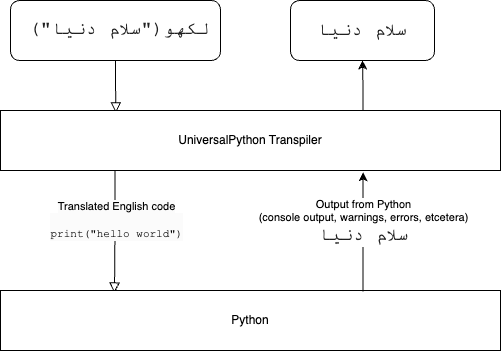
\includegraphics[width=\columnwidth]{UniversalPython-flowchart.png}}
\caption{A high-level abstraction of how the UniversalPython transpiler works.}
\label{flowchart}
\end{figure}

For example, if the user writes the following code in Urdu\footnote{Throughout this paper, we take the example of \textit{Urdu} (\texturdu{اردو}), the national language of Pakistan (the author's home country), and a traditional Right-to-left language, as an example translation language. }:


\begin{urdu} % Begin Urdu text block
\urdufont 
کچھ = ۲

اگر کچھ == ۱:

\quad لکھو ("سلام دنیا")

ورنہ:

\quad لکھو ("خدا ہافظ")

\end{urdu} % End Urdu text block

This is passed to “UniversalPython”, which first translates the code to English using Lexical Analysis and Parsing with the PLY library.
To do this, it first loads the Urdu dictionary, which is a YAML file containing mappings from Urdu to English. This dictionary is a mapping of each Urdu word to a Python keyword. Here is an example of such a dictionary:
In PLY, we have the option to reserve some keywords so that the library automatically tokenizes them. We set a Grammar Rule which, whenever a reserved keyword (i.e. a word which is present as a key in a language dictionary) is tokenized, simply looks for the token in the language dictionary (key) and replaces it with the corresponding English keyword (value).
We also set a Grammar Rule to ignore all content within double quotes or single quotes (i.e. strings and docstring) and to ignore content in comments (which start with a \#). We achieve this using Regular Expressions.
Urdu numbers also lie on the Unicode scale. \texturdu{۰} (or roman 0) is at 1776, while \texturdu{۹} (or roman 9) is at 1785.

Keeping this in mind, we define a Regular Expression which detects any symbols equal to or between this range, 1776 - 1785. These are the Urdu digits. We then use the same language dictionary to translate these numbers into roman numerals. For example, \texturdu{۵} becomes 5, \texturdu{۹۰} becomes 90, \texturdu{۱۰} becomes 10, \texturdu{۲۰۲۵} becomes 2025.
Furthermore, we also replace all periods ( . ) and commas ( , ), as these look different in Urdu than they do in English.

The rest of the code remains untouched. Whether it is a symbol like :, ;, etc, or even if it causes the lexer to crash, we ignore it so we can preserve the original structure of the code as much as possible. It is not required to translate such symbols and errors anyway; They are meant to be handled by Python, not UniversalPython. Back to our initial example code, our transpiler detects and replaces it with print , \texturdu{اگر} is replaced with if,
\texturdu{ورنہ} is replaced with else, and all Arabic digits are replaced with Roman digits. Hence the translated code would be:

\begin{lstlisting}
khchh = 2
if khchh == 1:
  print ("helloworldurdu")
else:
  print ("goodbyeurdu")
\end{lstlisting}

The above code is essentially vanilla Python code which can now simply be executed by the Python interpreter. The Urdu variable name was auto-translated to English using the unidecode library, however, even  does not present any issue to Python, as from Python 3.0 onwards, Unicode is fully supported. So the above code is passed on to the Python interpreter. The Python interpreter outputs some response; it can be some print statements which the user entered, compiler/interpreter warnings, and/or errors. This response is passed up to UniversalPython, where again it is tokenized to replace keywords in case of error messages. In our example, since there are no errors, it simply outputs the response as-is. So the response would be:

\begin{urdu} % Begin Urdu text block
\urdufont 
سلام دنیا

\end{urdu} % End Urdu text block
  

To demonstrate the ease by which plugins can be made for UniversalPython, we made a wrapper for the IPython kernel in which we imported UniversalPython as a package, and processed the code (i.e. translated it from Urdu to English) before it was passed onto IPython. This way, we overrode the functions and achieved a working kernel for UniversalPython. It works line-by-line while maintaining the program memory. This also gave us a visual interface for the language to test it thoroughly.

\begin{table}[h]
    \centering
    \caption{Language dictionary for periods and commas}
    \label{tab:language_dictionary}
    \begin{tabular}{cc}
    \hline
    Key & Value \\
    \hline
    . & \texturdu{۔} \\
    , & \texturdu{،} \\
    \hline
    \end{tabular}
    \end{table}

The Urdu dictionary is a YAML file containing mappings from Urdu to English keywords, is used for translation. The PLY library allows reserving keywords for automatic tokenization and replacement with their English equivalents. Additionally, grammar rules are set to ignore content within quotes, comments, and Urdu numbers (which lie on the Unicode scale).

\begin{table}[h]
    \centering
    \begin{tabular}{|c|c|}
    \hline
    Python (original) & Urdu (\texturdu{اردو}) \\
    \hline
    `print` & \texturdu{لکھو} \\
    `if` & \texturdu{اگر} \\
    `elif` & \texturdu{ورنہاگر} \\
    `else` & \texturdu{ورنہ} \\
    `while` & \texturdu{جبتک} \\
    `for` & \texturdu{جو} \\
    `in` & \texturdu{اندر} \\
    `input` & \texturdu{داخله} \\
    `break` & \texturdu{توڑ} \\
    `continue` & \texturdu{جاری} \\
    `pass` & \texturdu{گزر} \\
    `True` & \texturdu{حق} \\
    `False` & \texturdu{باطل} \\
    \hline
    \end{tabular}
    \caption{Comparison of Python Keywords and their Urdu Equivalents}
    \label{tab:python_urdu}
    \end{table}

    
\section{Experimentation}

\subsection{Evaluation metrics}\label{AA}

We propose the following metrics which UniversalPython should meet in order than it is considered effective:

1) Programs which work in Python, should work in UniversalPython.

2) UniversalPython should operate as a reasonable speed which at least does not disturb the programmer.

3) UniversalPython should be able to translate from one non-English language to another

4) A comparison should be made against other existing non-English, monolingual programming languages and multilingual programming languages

5) A user experience test should be conducted to find out user acceptability towards a language in their native tongue.

\subsection{Benchmarks with Python}\label{BB}

\textbf{Time:} Check the execution time / performance of Python vs UniversalPython. We use a benchmarking tool called hyperfine which runs each program multiple times to produce a mean execution time.

\textbf{Conversion:} Convert simple programs from English Python to UniversalPython, and test if they still work. Our testing mechanism for the above is as below:

1) We take an existing Python program, lets say multiplication.py.

2) Run the UniversalPython system in reverse. This will flip the language dictionary and generate an Urdu version of the program (all the keywords would be translated from English to Urdu). Save it as multiplication.ur.py.

3) Run multiplication.ur.py using UniversalPython, and multiplication.py using Python.

If both give the same output on the terminal then no data loss has occurred; Both Urdu program and English program output the same message. Hence we can say that the program has safely converted from English to UniversalPython and vice versa without breaking the code or changing the logic.

We take simple algorithmic programs from TheAlgorithms/Python \cite{thealgorithms_python}, a repository containing implementations of well-known algorithms, in the Python programming language. We run a loop over them and run the above algorithm on each to test.

Our framework allows easy support for UniversalPython plugins in existing Python IDEs. It acts as a bridge, translating Urdu code into English before passing it to the IDE.


\section{Results}


\subsection{Benchmarking Python and UniversalPython code}

We evaluate the results of the experiment mentioned above in the following two ways:
Execution Success Rate After running the experiment, we were able to achieve the following results.


\begin{table*}[t]
    \caption{Comparing UniversalPython with other non-English, monolingual programming languages and multilingual programming languages using "A Framework for the Localization of Programming Languages" \cite{swidan2023framework} }
    \centering
    \begin{tabularx}{\textwidth}{l *{14}{c}}
    \hline
    Aspect/Prog Language & UniversalPython & Scratch & Snap! & Dolittle & Ebda3 & Qalb & Wenyan & Excel & PSeInt & Rapture & Hedy & Hindi & Linotte \\
    \hline
    Language & Multi & Multi & Multi & Japanese & Arabic & Arabic & Chinese & Multi & Spanish & Russian & Multi & Hindi & French \\
    Alignment & N & N & N & N & N & T & N & T & N & T & NT & N & N \\
    Non-English keywords & $\bullet$ & $\bullet$ & $\bullet$ & $\bullet$ & $\bullet$ & $\bullet$ & $\bullet$ & $\bullet$ & $\bullet$ & $\bullet$ & $\bullet$ & $\bullet$ & $\bullet$ \\
    Non-Latin variable names & $\bullet$ & $\bullet$ & $\bullet$ & $\bullet$ & $\bullet$ & $\bullet$ & $\bullet$ & $\circ$ & $\bullet$ & $\bullet$ & $\bullet$ & $\bullet$ & $\bullet$ \\
    Non-English productions & $\bullet$ & $\circ$ & $\bullet$ & - & - & $\bullet$ & $\circ$ & $\bullet$ & - & - & - & $\bullet$ & - \\
    Non-English numerals & $\bullet$ & - & - & - & - & $\bullet$ & $\bullet$ & $\bullet$ & - & - & $\bullet$ & - & - \\
    Characters without meaning & $\bullet$ & - & - & - & - & $\bullet$ & $\bullet$ & - & - & - & $\circ$ & - & - \\
    Diacritics & $\bullet$ & $\bullet$ & $\bullet$ & $\circ$ & $\circ$ & $\bullet$ & $\circ$ & - & $\bullet$ & $\circ$ & $\bullet$ & $\bullet$ & $\bullet$ \\
    Alternative keywords & $\bullet$ & - & - & - & $\circ$ & - & $\bullet$ & - & $\bullet$ & $\circ$ & $\bullet$ & - & - \\
    Localized punctuation & $\bullet$ & $\circ$ & $\circ$ & $\circ$ & $\circ$ & $\circ$ & $\bullet$ & $\bullet$ & - & - & $\bullet$ & - & - \\
    Right to left support & $\bullet$ & $\circ$ & - & $\circ$ & $\bullet$ & $\bullet$ & $\circ$ & $\bullet$ & - & - & $\bullet$ & $\circ$ & $\circ$ \\
    Multi-lingual programming & $\bullet$ & - & - & - & - & - & - & - & - & $\bullet$ & $\circ$ & - & - \\
    Error messages & - & $\circ$ & $\circ$ & $\bullet$ & $\circ$ & $\circ$ & - & $\bullet$ & $\bullet$ & - & $\bullet$ & $\bullet$ & $\bullet$ \\
    Multi-lingual 3rd-party libraries & $\circ$ & $\circ$ & - & $\circ$ & $\circ$ & $\circ$ & $\circ$ & $\bullet$ & - & - & $\bullet$ & $\bullet$ & $\bullet$ \\
    \hline
    \end{tabularx}
    \end{table*}
    

“Table III“ describes our results over 110 simple Python programs present in TheAlgorithms/Python [14] maths implementation.
We reported that 98\% of simple programs can be automatically converted into Urdu Python without breaking the code. Amongst the programs that failed, the reason was due to a problem in generating the Urdu version of an English program (i.e. running UniversalPython in reverse) - it cannot distinguish between “is” and “==”, as they have the same purpose in English Python.
Execution Time Upon recording the execution time summary of the experiment we concluded that UniversalPython performed better with simpler and less wordy programs, whereas for more wordy and lengthy algorithms, python performed better in terms of execution time. However, it is well within the range of acceptable speed of a programming language. Some of the top differences in performances of some algorithms can be seen in the tables “Table IV“ and “Table V“.
Table IV: Execution times of functions where our transpiler performed well.

\subsection{Trying out different languages and translating between them}

It is possible to make this framework generic \textit{enough} to span multiple languages. We managed to make three variants; Urdu, Chinese and Hindi, to demonstrate UniversalPython's capability to extend multiple languages.

We were then able to translate between languages, e.g. Urdu to Hindi (as shown in Figure \ref{language-to-language}), by using English as an \textit{intermediate language}.

\begin{figure}[htbp]
\centerline{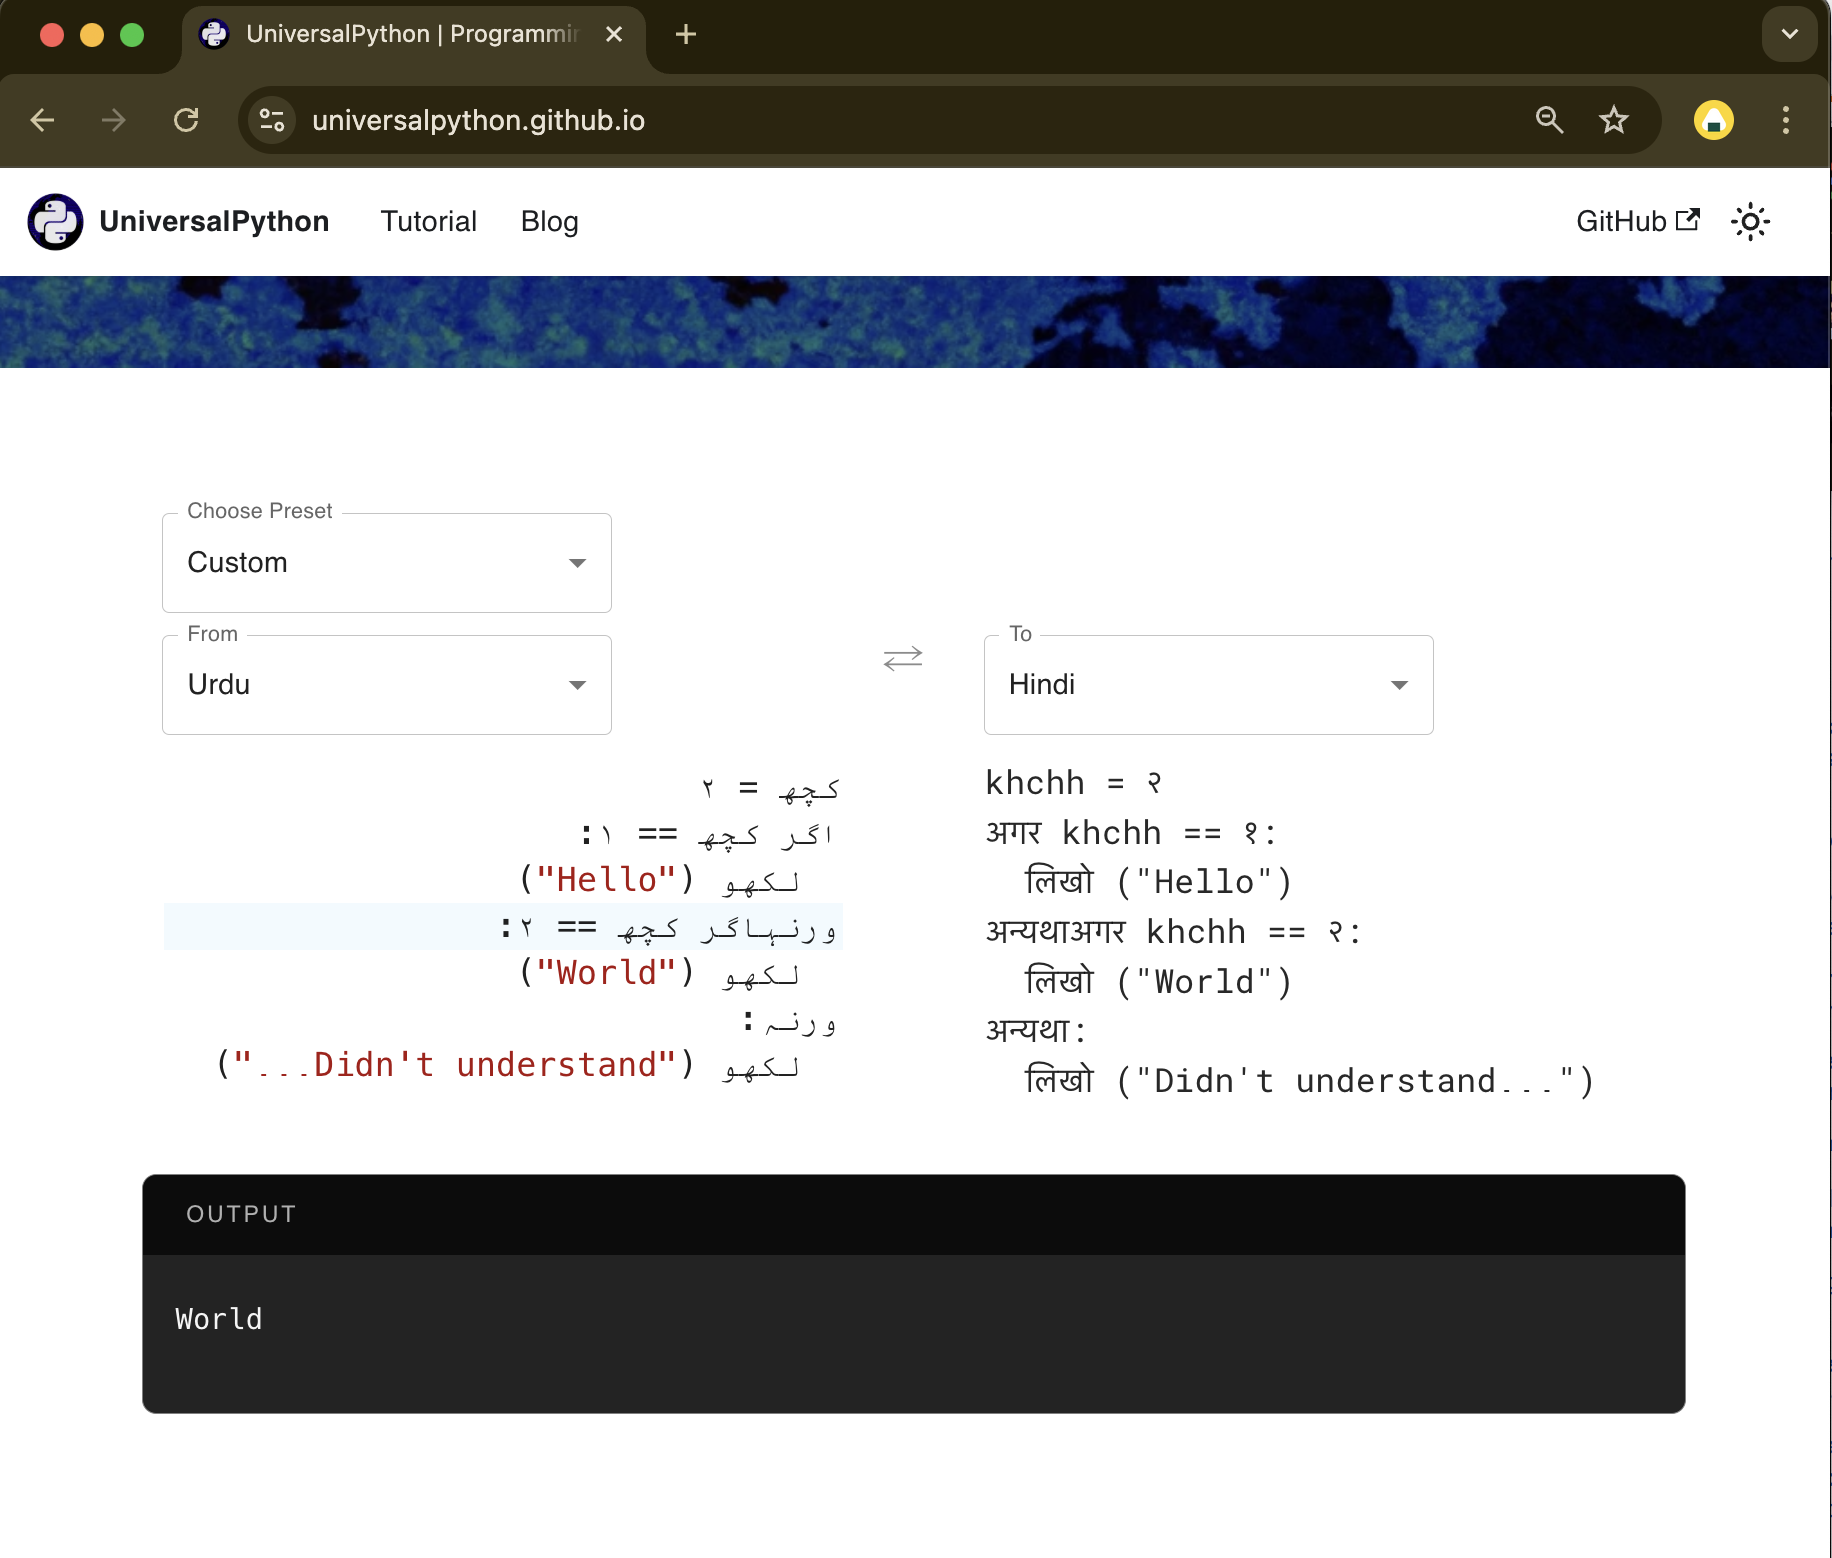
\includegraphics[width=\columnwidth]{UniversalPython-language-to-language.png}}
\caption{Urdu to Hindi code translation and successful compilation with UniversalPython.}
\label{language-to-language}
\end{figure}

\subsection{Making the Jupyter Kernel}

To demonstrate the ease by which plugins can be made for UniversalPython, we made a wrapper for the IPython kernel in which we imported UniversalPython as a package, and processed the code (i.e. translated it from Urdu to English) before it was passed onto IPython. This way, we overrode the \verb|do_execute| and \verb|do_complete| functions and achieved a working kernel for UniversalPython. It works line-by-line while maintaining the program memory. This also gave us a visual interface for the language to test it thoroughly.

\section{Limitations}

- Third-party library support is vital for any software platform to flourish. While third-party libraries do not cause the program to crash, we would prefer a better developer experience in which third-party libraries are also translated.

- It is currently not possible translate words with spaces in between them. For example, `elif` in Python actually translates to \texturdu{ورنہ اگر} (notice the space in the middle) in the Urdu language. Some languages may also have different placements for verbs and nouns, and different words for different quantities (e.g. mono, bi, tri). This may present a challenge for UniversalPython, where more creative effort may be needed to construct a better front-end experience for programmers, while ensuring compatibility with Python.

- Translation quality is very weak for certain low-resources and contextual languages.


\section{Future Work}

UniversalPython can be developed as an extensible programming language which would grow alongside Python and would be interoperable with it. It is also maintainable, because since it is simply a wrapper, only the keywords need to be updated in the dictionary, and it will work for any future (or past) versions of Python. Furthermore, it is scalable to other languages because the dictionary structure allows for any language to be added to UniversalPython.

To improve the current implementation, it would be useful to accommodate as many Python keywords as possible, preferably all of them. It would also be useful to separately have translations for major libraries/packages such as pandas, numpy, cv2, etc. A scalable and efficient method for this would be to automatically scan such libraries (the Python source code) to identify important keywords, automatically translate them to the nearest and best possible Urdu word, and add them to the Grammar. This can be achieved using Natural Language Processing, Deep Learning, Machine Learning and similar methods.

This framework could take on a similar role as TypeScript does in the JavaScript world, where it is usually used as a build-time transpiler to JavaScript \cite{Understanding_TypeScript}. To make it easy for third-party libraries to integrate with UniversalPython, inspiration can be taken from TypeScript's {\em *.d.ts} files --- in UniversalPython's case, it could be an {\em interfaces.<language\_code>.yml} file containing the translations for the functions and variables, in a predefined format. Again, we leave this to the imagination of the reader.

In the current framework, making it possible for the user to \textit{choose} whether or not to detect variables and functions, and translate them with machine translation into their corresponding names, could make the experience better.

In order to increase the accuracy of the translations, a translation-verification system can be developed, where beginner and experienced programmers can be asked, "How would you write the following snippet of code in your language?", and let them write the code in any shape or form they desire. This could be done with data from platforms like Leetcode, however, we leave that to the imagination of the reader.

It would also be helpful to conduct more User Experience tests with programmers across the globe, so that it can be determined whether or not UniversalPython really does benefit people who speak non-English languages to learn programming.

Designing and developing a better evaluation metric to test the effectiveness of UniversalPython and similar multilingual programming languages / frameworks.

A REPL can be made by hooking into the Python REPL. Integrations can be made with Replit, Leetcode etcetera.

Support from official Python could boost the project a lot.

\section*{Acknowledgment}

I would like to acknowledge my mentor, Dr Omer Beg, for always guiding me to the right path during my Bachelor's, professional life, and Master's degree.

\bibliographystyle{bibtex/IEEEtran} % Or your desired style (e.g., IEEEtran)
\bibliography{bibtex/IEEEexample} 

\vspace{12pt}
\end{document}
